\documentclass{standalone}
\usepackage{graphicx}
\usepackage{tikz}

\usetikzlibrary{shapes.geometric, arrows, positioning, calc}
\tikzset{
  to/.style  = {->, >=stealth', shorten >=1pt, thin, draw=#1, fill=#1}
}

\begin{document}
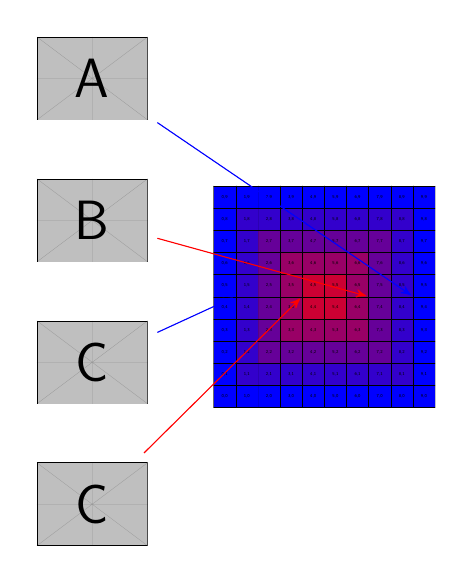
\begin{tikzpicture}
    \node[anchor=south west,inner sep=0] (image) at (0,0,0) {\includegraphics[width=80pt]{example-grid-100x100pt}};
    \node[above left=1cm of image] (one) {\includegraphics[width=40pt]{example-image-a}};
    \node[below=0.5cm of one] (two) {\includegraphics[width=40pt]{example-image-b}};
    \node[below=0.5cm of two] (three) {\includegraphics[width=40pt]{example-image-c}};
    \node[below=0.5cm of three] (four) {\includegraphics[width=40pt]{example-image-c}};

    \begin{scope}[x={(image.south east)},y={(image.north west)}]
    \iffalse
        \draw[help lines,xstep=.1,ystep=.1] (0, 0) grid (1, 1);
        \draw[help lines,xstep=.05,ystep=.05] (0, 0) grid (1, 1);
        \foreach \x in {0,1,...,9} { \node [anchor=north] at (\x/10,0) {0.\x}; }
        \foreach \y in {0,1,...,9} { \node [anchor=east] at (0,\y/10) {0.\y};}
        \fi
        \begin{scope}
			\draw[to=blue] (one)   -- (0.9,0.5);
            \draw[to=red]  (two)   -- (0.7,0.5);
            \draw[to=blue] (three) -- (0.1,0.5);
            \draw[to=red]  (four)  -- (0.4,0.5);
        \end{scope}
    \end{scope}
\end{tikzpicture}
\end{document}
